\section*{Part 1 [25 points]}

Using the instructions provided in the project description, run memcached alone (i.e., no interference), and with each iBench source of interference (cpu, l1d, l1i, l2, llc, membw). For Part 1, you must use the following \texttt{mcperf} command, which varies the target QPS from 30000 to 110000 in increments of 5000 (and has a warm-up time of 2 seconds with the addition of \texttt{-w 2}):

\begin{verbatim}
$ ./mcperf -s MEMCACHED_IP --loadonly
$ ./mcperf -s MEMCACHED_IP -a INTERNAL_AGENT_IP  \
           --noload -T 16 -C 4 -D 4 -Q 1000 -c 4 -w 2 -t 5 \ 
           --scan 30000:110000:5000
\end{verbatim}

\noindent Repeat the run for each of the 7 configurations (without interference, and the 6 interference types) \textbf{at least three times} (three should be sufficient in this case), and collect the performance measurements (i.e., the \texttt{client-measure} VM output). Reminder: after you have collected all the measurements, make sure you \underline{delete your cluster}. Otherwise, you will easily use up the cloud credits. See the project description for instructions how.

%%%%%%%%%%%%%%%%%%%%%%%%%%%%%%%%%%%%%%%%%%%
%%% QUESTION 1A

\begin{enumerate}[label=(\alph*)]
    \setcounter{enumi}{0}

    \item \textbf{[10 points]} Plot a single line graph with the following stipulations:
    \begin{itemize}
        \item Queries per second (QPS) on the x-axis (the x-axis should range from 0 to 110K).\\
        (note: the actual achieved QPS, not the target QPS)
        \item 95th percentile latency on the y-axis (the y-axis should range from 0 to 8 ms).
        \item Label your axes.
        \item 7 lines, one for each configuration. Add a legend.
        \item State how many runs you averaged across and include error bars at each point in both dimensions.
        \item The readability of your plot will be part of your grade.
    \end{itemize}
    
    % \textbf{The shape of the curves depends on many factors and may differ across groups. However, that does not imply that your solutions are wrong.}
    \textbf{Solution:} In order to plot the graph we averaged three different runs: as we only have three measurements the error bars represent the minimum and maximum measurements taken, while the point represents the average. We could represent the error bars as the standard deviation but with our approach we do not lose information in the measurements as they are represented directly in the graph. For the sake of readability, we averaged several measurements with achieved QPS very similar one to another in the \texttt{l1i} and \texttt{cpu} benchmarks as they struggle to reach more than 50K we would have an agglomerate of points there. In this way, we do not have too many points concentrated in the same area of the graph thus improving readability. This is also the reason why the error bars are bigger in this part of the graph as we are averaging over several results.

    \begin{figure}[!ht]
    \centering
    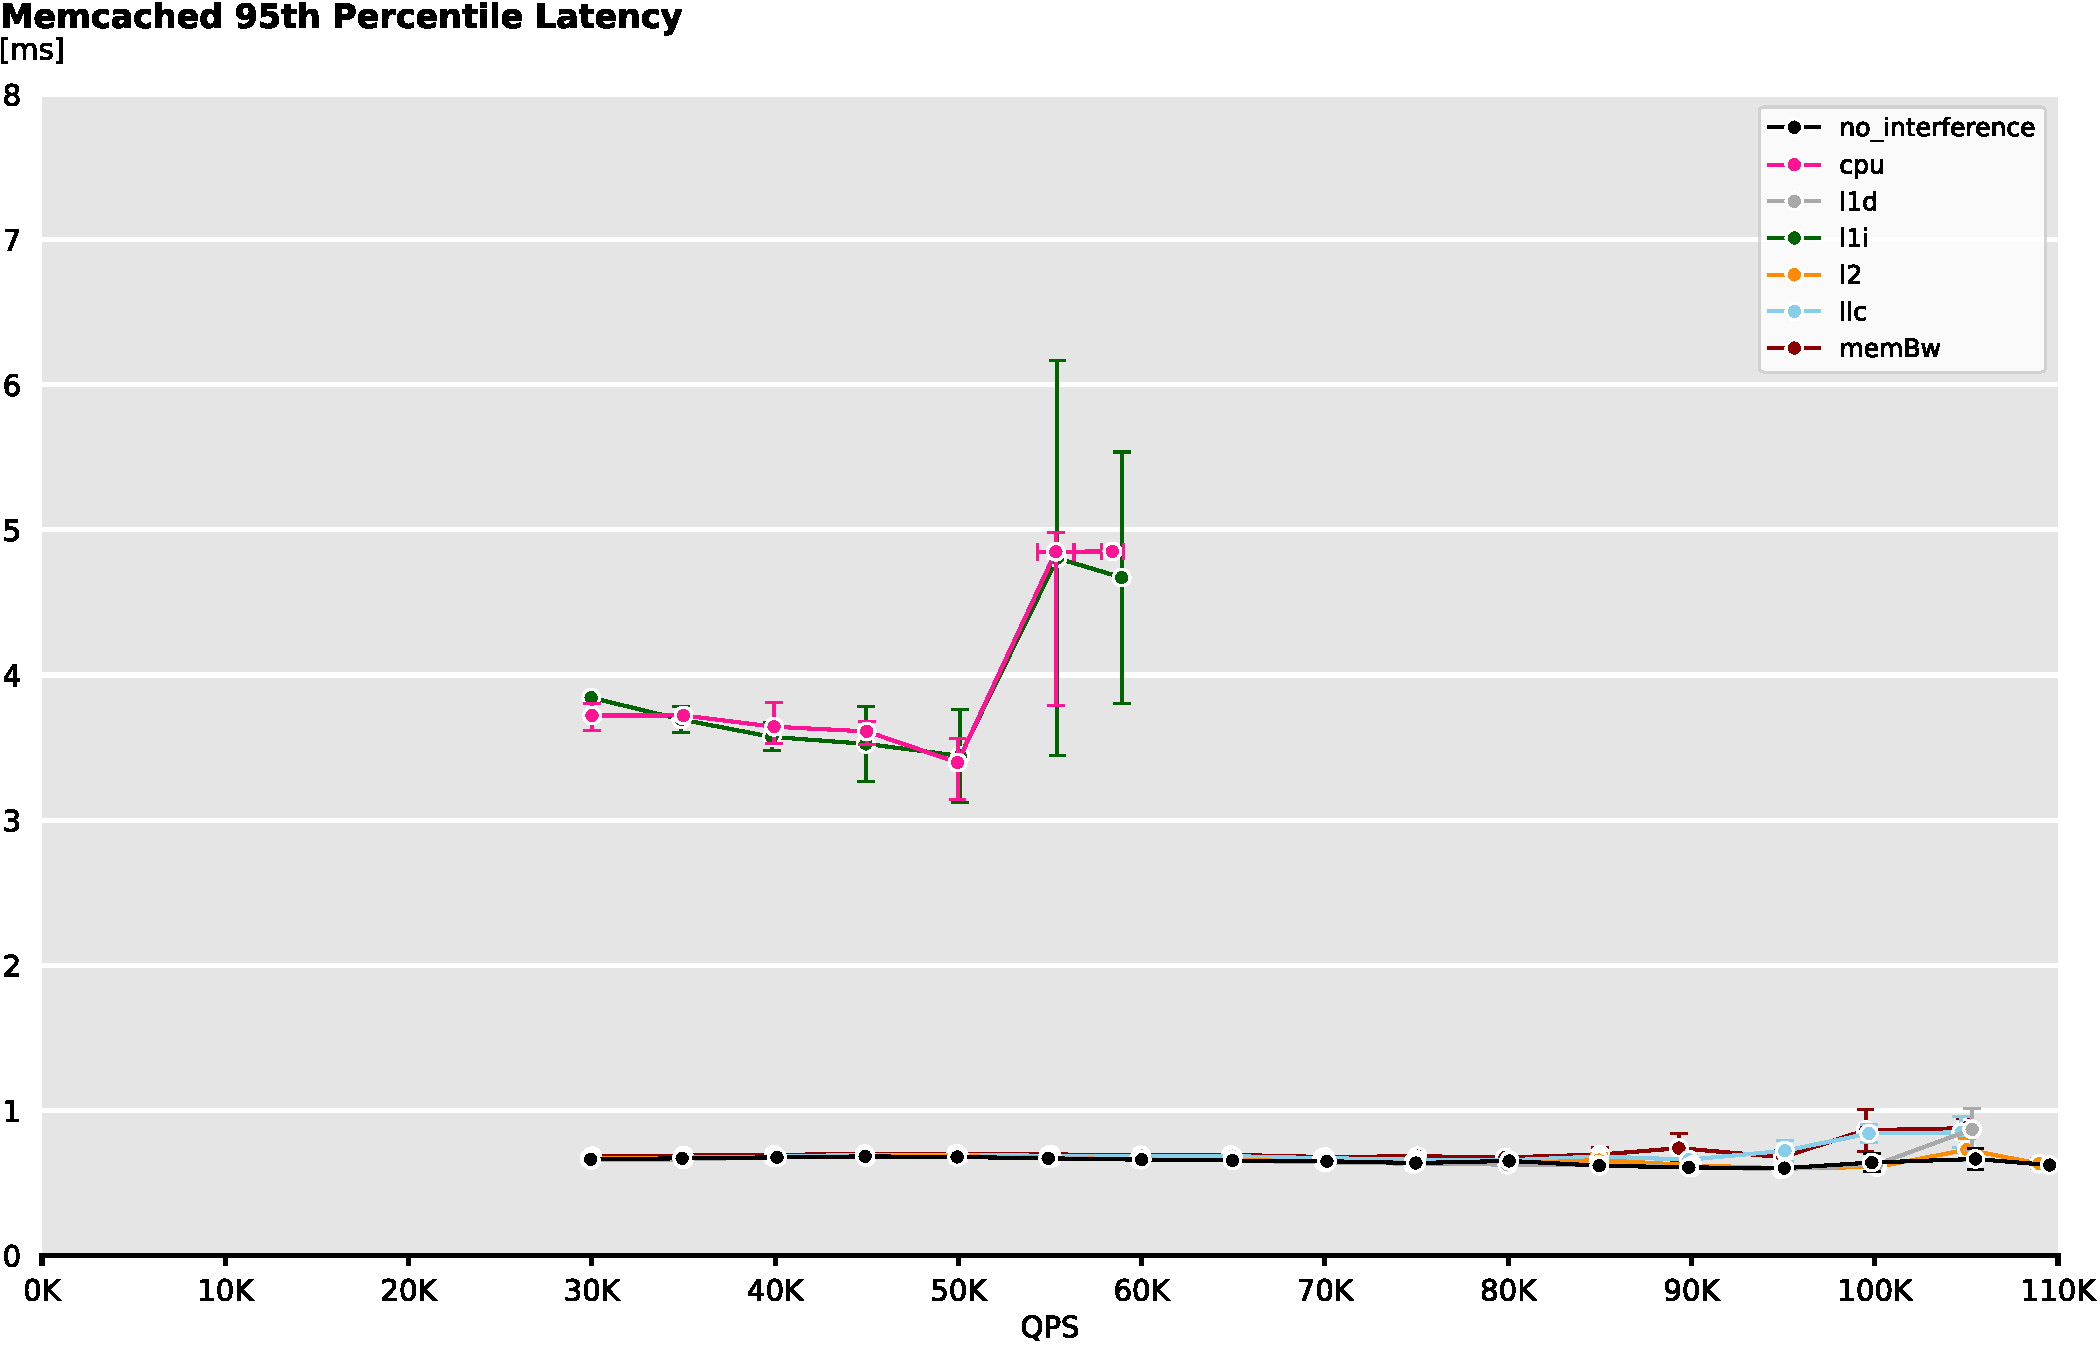
\includegraphics[width=\textwidth]{figures/plot1_total.pdf}
    \caption{\label{fig:plot1} 95th Percentile Latency}
    \end{figure}

    \newpage
    
    
\end{enumerate}



% Here you place your solution.

%%%%%%%%%%%%%%%%%%%%%%%%%%%%%%%%%%%%%%%%%%%
%%% QUESTION 1B

\begin{enumerate}[label=(\alph*)]
    \setcounter{enumi}{1}
    
    \item \textbf{[6 points]} How is the tail latency and saturation point (the “knee in the curve”) of memcached affected by each type of interference? Why? Briefly describe your hypothesis.
    
    \textbf{Solution:} \textbf{memcached} reaches saturation point around 55K with \texttt{cpu} and \texttt{l1i} benchmarks. From time to time it manages to get to 60K QPS, but this is anecdotal. Therefore, we can conclude that \textbf{memcached} makes a huge use of CPU operation and has to process lots of instructions.
    
    The application seems to be less memory dependent as \texttt{l1d},  \texttt{l2}, \texttt{llc} and \texttt{memBW} have a much smaller latency even if texttt{llc} and \texttt{memBW} start to get a slightly bigger latency at 90K. This is at first glance unexpected as \textbf{memcached} is by definition using the memory to cache database values and has to retrieve them frequently. In fact \texttt{memBW} and \texttt{llc} have the worst performance among this group of benchmarks, which point to the mentioned memory dependency. \texttt{l1d}, \texttt{llc} and \texttt{memBW} seem to reach the saturation point at 105K which may indicate that higher QPS could lead to a big drop in performance. All in all, our hypothesis for this better than expected performance is that the memory bandwidth in the VM is big enough to handle the transfer of the small chunks of data that \textbf{memcached} retrieves from memory. 
    
\end{enumerate}

%%%%%%%%%%%%%%%%%%%%%%%%%%%%%%%%%%%%%%%%%%%
%%% QUESTION 1C

\begin{enumerate}[label=(\alph*)]
    \setcounter{enumi}{2}
    
    \item \textbf{[2 points]} Explain the use of the \texttt{taskset} command in the container commands for memcached and iBench in the provided scripts. Why do we run some of the iBench benchmarks on the same core as memcached and others on a different core?

    
     \textbf{Solution:} \texttt{taskset} allows to set the core on which each benchmark will be run, more precisely it uses a mask to specify the processor affinity of a process, that is the set of CPUs a thread is eligible to run on. Thus we can divide the benchmark in two groups, the one that have to run on the same core as memchached and the one that aren't supposed to. It is straightforward to conclude that we should run the \texttt{cpu} benchmark on the same core of \textbf{memcached}, as the task of this benckmark is to strain the CPU. Furthermore, \texttt{l1i}, \texttt{l1d} and \texttt{l2} are not shared among cores so they also have to be run in the same core as the one used by the application that wants to be tested. Nevertheless, they are not really CPU intensive so they don't create additional interference. On the other hand, \texttt{llc} and \texttt{memBW} can and should be run on a separate core as these resources are shared among cores and these benchmarks are more CPU intensive and this would create addditional interference.
    
\end{enumerate}

% Here you place your solution.

%%%%%%%%%%%%%%%%%%%%%%%%%%%%%%%%%%%%%%%%%%%
%%% QUESTION 1D
    
\begin{enumerate}[label=(\alph*)]
    \setcounter{enumi}{3}
    
    \item \textbf{[2 points]} Assuming a service level objective (SLO) for memcached of up to 1.5~ms 95th percentile latency at 65K QPS, which iBench source of interference can safely be collocated with memcached without violating this SLO? Briefly explain your reasoning.

    \textbf{Solution:} Taking a look at the graph we can see that at 65K QPS \texttt{l1i} and \texttt{cpu} cannot be collocated with memcached without violating the SLO of up to 1.5~ms 95th percentile given that they are well above that time limit, around 5 ms. They even struggle to process more than 50K QPS. \texttt{l1d},  \texttt{l2}, \texttt{llc} and \texttt{memBW} can be safely collocated as they are below 1 ms of tail latency, and do not struggle processing any number of QPS.
            
\end{enumerate}

% Here you place your solution.

%%%%%%%%%%%%%%%%%%%%%%%%%%%%%%%%%%%%%%%%%%%
%%% QUESTION 1E
    
\begin{enumerate}[label=(\alph*)]
    \setcounter{enumi}{4}
    
    \item \textbf{[5 points]} In the lectures you have seen queueing theory. Is the project experiment above an open system or a closed system? What is the number of clients in the system? Sketch a diagram of the queueing system and provide an expression for the average response time. Explain each term in the response time expression.

    \textbf{Solution:} This is clearly a closed system as the number of clients is well established. Based on the manual of memcache-perf we can see that we are running a total of 16 thread (\texttt{-T 16}) and each one of these threads open a total of 4 connections (\texttt{-C 4}) from the VM client-agent to the \textbf{memcached} server. One additional connection is opened in the client-measure VM that is in charge of taking the measurements. Therefore, the \textbf{total} number of clients is \textbf{65}. It is also stated in the manual that mcperf "waits for a reply before sending the next request". All in all, this makes it a closed system by definition.
    
    In Figure \ref{fig:plot1} the queueing system of the described closed system is represented.

    \begin{figure}[!h]
    \centering
    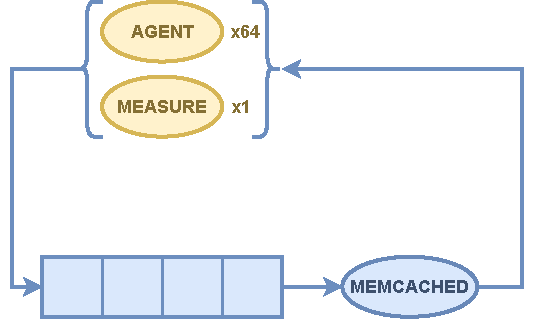
\includegraphics[width=0.5\textwidth]{figures/Untitled Diagram-Page-3.drawio.pdf}
    \caption{\label{fig:plot1} Queueing system}
    \end{figure}

    The expression for the average response time ($R$) is included below:

    $$R = \frac{N}{X} - Z$$

    $N$ represents the number of clients in the closed system and $Z$ represents the think time of the clients. In other words $Z$ represents the possible delay between a client receiving an answer from the server and the time it sends the next request. In our case, if a think time is present in the clients, it would have to be really small as we limit the total runtime of sending and receiving requests to 5 seconds (\texttt{-t 5}). Finally, $X = \frac{Jobs}{Time}$ is the throughput or number of queries per second.
            
\end{enumerate}

% Here you place your solution.
\
